\documentclass[11pt]{article}

\usepackage[margin=1in]{geometry}
\usepackage{fancyhdr}
\pagestyle{fancy}
\usepackage{amsmath}
\usepackage{amssymb}
\usepackage{multirow}
\usepackage{array}
\usepackage{tikz}
\usetikzlibrary{calc,trees,positioning,arrows,fit,shapes,calc}

\lhead{Proofs}
\chead{Asli Akalin | Note 2}
\rhead{Summer 2018}


\begin{document}

\section*{Review Questions}
\begin{enumerate}
\item If chemical plant pollutes river, fish die. If fish die, did the chemical plant pollute water?
\item Are these statements logically equivalent? a) If plant pollutes, fish die. b) if fish die, plant pollutes.
\item $(\forall x \in Z) (\exists y \in Z) (y > x)$? $(\exists y \in Z) (\forall x \in Z)  (y > x)$?
\end{enumerate}

\section*{Answers}
\begin{enumerate}
\item First, define P(x) as "chemical plant pollutes water" and Q(x) as "fish die." We have "if chemical plant pollutes river, fish die" known to be True: $P(x) \Rightarrow Q(x) \equiv T$. The question asks if fish die, $Q(x) \equiv T$, did the chemical plant pollute the water, $P(x) \equiv T$? Using the implication definition, we know that $P(x) \Rightarrow Q(x)$ and $Q(x)$ True can mean $P(x)$ is either True or False, since $T \Rightarrow T$ and $F \Rightarrow T$ both evaluate to T. So, by knowing fish died and knowing one of the reasons fish dies is chemical plant pollution, we cannot conclude that chemical plant polluted the water. Intuitively, we can see that fish might have died from a different reason. So, the fact that fish died does not necessarily mean chemical plant pollutes water. 
Key Point: P is sufficient for Q (proving P allows you to conclude Q is true, since if $P \rightarrow Q$ is true and P is true, Q has to be true) but Q is necessary for P (for P to be true Q is required to be true, because if $P \rightarrow Q$ is true and Q is false, P has to be false to make the implication still be true).
\item They are not logically equivalent. They are the converse of each other. If plant pollutes, fish will die for sure, so if fish are alive it is safe to say plant is not polluting. But fish can die for many reasons, so just because fish die we can't be certain that plant is polluting. (Exercise inception: prove these explanatory sentences using logic language.)
\item Frist statement says for each integer x, we can find at least one integer y that is bigger than x. True since there is always a bigger integer. Second statement says that there is one integer, call it y, such that it is bigger than all integers. False since there is no "biggest integer"
\end{enumerate}

\newpage
\section*{Graphing Technique for Evaluating Quantifiers}
\begin{enumerate}
\item
\begin{figure}[ht]
\centering
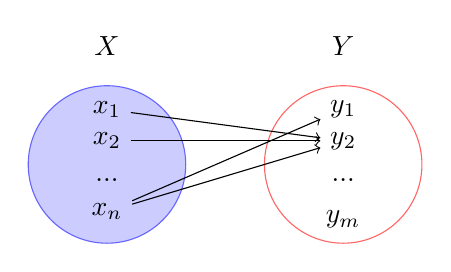
\begin{tikzpicture}
    % draw the sets
    \filldraw[fill=blue!20, draw=blue!60] (-1.5,0) circle (1cm);
    \filldraw[fill=red!0, draw=red!60] (1.5,0) circle (1cm);

    % the texts
    \node at (-1.5,1.5) {$X$};
    \node at (1.5,1.5) {$Y$};

    % the points in the sets (here I just create nodes to use them later on to position
    % the circles and the arrows
    \node (x1) at (-1.5,0.7) {$x_1$};
    \node (x2) at (-1.5,0.3) {$x_2$};
     \node (x3) at (-1.5,-0.2) {$...$};
    \node (x4) at (-1.5, -0.6) {$x_n$};
    \node (y1) at (1.5,0.7) {$y_1$};
    \node (y2) at (1.5,0.3) {$y_2$};
    \node (y3) at (1.5,-0.2) {$...$};
    \node (y4) at (1.5,-0.7) {$y_m$};

    % draw the arrows
    \draw[->] (x1) -- (y2);
    \draw[->] (x2) -- (y2);
    \draw[->] (x4) -- (y2);
    \draw[->] (x4) -- (y1);

\end{tikzpicture}
\caption{Mapping diagram of ($\forall x$, $\exists y$) for some statement P(x,y)}
\end{figure}
\begin{enumerate}
\item $\forall x$ makes sure all x are selected in set of x, for each $x_i$ there will be (at least one) arrow going out, this set of X is all selected. Therefore we can say for all x, there at least some y (one or more) that makes P(x,y) True.
\item $\forall x$, $\exists y$ does not guarantee that all y values in set Y will have a corresponding x value to make statement P(x,y) true, for example in this example $y_m$ doesn't have a x pair. \newline$\forall x$, $\exists y$ means all $x_i$ can point at the same y value, or different y values.
\item Only thing known for certain here is that you can pick any x value, and you can find a specific y' value for that x make $P(x, y')$ correct, $y'$ can be the same for all x or each x might use different y values.
\end{enumerate}



\begin{figure}[ht]
\centering
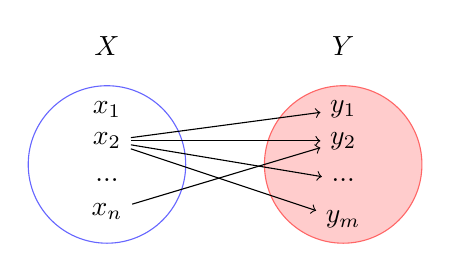
\begin{tikzpicture}
    % draw the sets
    \filldraw[fill=blue!0, draw=blue!60] (-1.5,0) circle (1cm);
    \filldraw[fill=red!20, draw=red!60] (1.5,0) circle (1cm);


    % the texts
    \node at (-1.5,1.5) {$X$};
    \node at (1.5,1.5) {$Y$};

    % the points in the sets (here I just create nodes to use them later on to position
    % the circles and the arrows
    \node (x1) at (-1.5,0.7) {$x_1$};
    \node (x2) at (-1.5,0.3) {$x_2$};
     \node (x4) at (-1.5,-0.2) {$...$};
    \node (x5) at (-1.5, -0.6) {$x_n$};
    \node (y1) at (1.5,0.7) {$y_1$};
    \node (y2) at (1.5,0.3) {$y_2$};
    \node (y3) at (1.5,-0.2) {$...$};
    \node (y4) at (1.5,-0.7) {$y_m$};

    % draw the arrows
    \draw[->] (x2) -- (y1);
    \draw[->] (x2) -- (y2);
    \draw[->] (x2) -- (y3);
    \draw[->] (x2) -- (y4);
    \draw[->] (x5) -- (y2);

\end{tikzpicture}
\caption{Mapping diagram of ($\exists x$, $\forall y$) for some statement P(x,y)}
\end{figure}
\item 
\begin{enumerate}
\item $\exists x$ makes sure that there is (at least) one x, x' such that it can be paired with every single y value to make the statement P(x,y) correct. In this case the guarantee is that the set Y is covered.
\item $\exists x$, $\forall y$ doesn't mean there is only one x that can make P(x,y) correct. For example in this example $y_2$ can be paired with $x_2$ or $x_n$. 
\item However $\exists x$, $\forall y$ does enforce that if we took let's say $y_11$, $y_167$ and $y_4$, we would be able to find at least one specific x that can be paired with all those values to make P(x,y) correct.
\end{enumerate}
\item Be careful with what the order of quantifiers guarantee and what they might satisfy in certain cases!! For example $\exists x$, $\forall y$ might mean that there are two x values $x_i$ and $x_j$ such that all y values can be paired with either to make P(x,y) but it does not guarantee that some x, $x_k$ will have a corresponding y value to make P(x,y) correct. 
\end{enumerate}
\newpage
\section*{Proof Methods}
\begin{tabular}{ |m{10em}|m{10em}|m{11em}|m{11em}| } 
 \hline
 Direct Proof & by Contraposition & Contradiction & by Cases \\
 \hline 
 \hline
 $ P \Rightarrow Q $ & $ \neg Q \Rightarrow \neg P $ & $ P $ & $P$ \\ 
 \hline
 
 
Assume P, tweak stuff therefore get Q. & 
Assume $\neg Q$, tweak stuff, therefore get $\neg P$ & 
Assume $\neg P$, tweak stuff, show contradiction by showing that $\neg P \Rightarrow R$ and $ \neg P \Rightarrow \neg R$. Since the individual implications has to be True, $ \neg P \Rightarrow (R \wedge \neg R)$ has to hold. Notice $(R \wedge \neg R)) \equiv F$. So $ \neg P \Rightarrow F$ can only hold if $\neg P$ is false, ($F \Rightarrow F \equiv T$). So, $\neg P \equiv F \Rightarrow P \equiv T$. Thus P has to be T. & 
list all of exhaustive cases. \\

\hline 

-When you an use the info given with P to derive info that eventually leads you to Q & 
- When the info given from P is vague or hard to derive info from, assuming $\neg Q$ gives you more information and easier to derive conclusions from & -When there is only a single statement to be proven without an implication & -Usually when nothing else works\newline -But technically you can do all proofs using by cases, if you are determined enough. \\

\hline
Can use when: & Can use when: & Can use when: & Can use when: \\
- specific definitions given in P such as "perfect square," "odd," "divisible by 5" can be used as stepping stones to get to next step \newline
- Assuming P immediately gives you information about other variables in the question (such as for odd n, $n = m^2$, means m has to be odd etc) & 

- P doesn't give enough information to move forward, is to vague or hard to assume \newline - $\neg Q$ is easier to assume, use and expand from \newline 
- when P is "n bigger/smaller than 6" (covers all n bigger than 6, hard to build on) \newline 
- when $\neg Q$ is a simple statement that can easily be negated & 

- Mostly when there is a simple statement like "there exists," "there is," without an implicit implication \newline
- P is easy to negate and develop on: \newline
- "there are infinite prime numbers" $\rightarrow$ "there are finite prime numbers" $\rightarrow$ "there is a largest prime number" \newline
- "at least 2 people have same number of friends" $\rightarrow$ "nobody has same number of friends" $\rightarrow$ "everybody has a unique number of friends"  & 
- Either case a, or case b, or case c ... has to occur but it is not possible to know which one will. \newline
- Only can be used when all possible cases are known, so be careful with infinite sets. \newline
- For example, the values n can take in the set Natural Numbers can be separated into cases as n=0, n=1, n=2 ... (which is hard to take into account one by one) or as $n<4, n=4, n>4$ etc, so define cases carefully. \\ 
\hline
\end{tabular}


\newpage
\section*{Useful Notes}
\begin{enumerate}
\item Basic Negation Keypoints
\begin{enumerate}
\item everybody does P $\rightarrow$  there exists (at least one) person that does not P
\item there exists (at least one) n such that P $\rightarrow$ all n are (not P)
\item $A > B$ $\rightarrow$ $A<= B$ 
\end{enumerate}

\item To have a proof of "if and only if" have to show the original implication and its converse to be true. If converse holds for an implication$P \Rightarrow Q$, then $ P \equiv Q$.
\item Proof by contraposition relies on the fact that contraposition of an implication is logically equivalent to the original implication.
\item Contraposition proof is essentially the direct proof of contrapositive, the only difference is that you start by assuming a the negation of RHS. So, if the goal is to prove an implication, decide between direct proof or contraposition by deciding whether P or $\neg Q$ is easier to assume.
\item Proof by contradiction especially works well with proving something does not exist. Start by assuming that it does exist and show why it would break the universe if it did exist. (Key idea: assume negation to show some nonsense/contradiction, but since all the steps were legit based on that assumption, the only explanation is that the assumption itself was wrong)



\end{enumerate}


\end{document}
